\question{Замена переменной в определенном интеграле. Интегрирование по частям.}

Замена в определенном интеграле выполняется также, как и в неопределенном за
исключением смены пределов интегрирования. Более формально:

\begin{align*}
  \int_{a}^{b} f(x) \dd x = \int_{\alpha}^{\beta} f(\phi(t)) \phi'(t) \dd t \\
  \phi(\alpha) = a, \phi(\beta) = b
\end{align*}

Интегрирование по частям для определенных интегралов выполняется также, как и
для неопределенных:

\begin{align*}
  \int_{a}^{b} u \dd v = u v \bigg\vert_{a}^{b} - \int_{a}^{b} v \dd u
\end{align*}

Стоит отметить несколько свойств определенных интегралов для четных и нечетных
функций на симметричном промежутке

\begin{multicols}{2}
  \begin{lemma}
    Если \(f(x)\) нечетная функция, то

    \begin{equation*}
      \int_{-a}^{a} f(x) \dd x = 0
    \end{equation*}
  \end{lemma}
  
  \begin{lemma}
    Если \(f(x)\) четная функция, то
    
    \begin{align*}
      \int_{-a}^{a} f(x) \dd x = 2 \int_{0}^{a} f(x) \dd x
    \end{align*}
  \end{lemma}  
\end{multicols}

\begin{figure}[H]
\centering

\begin{subfigure}[b]{0.5\textwidth}
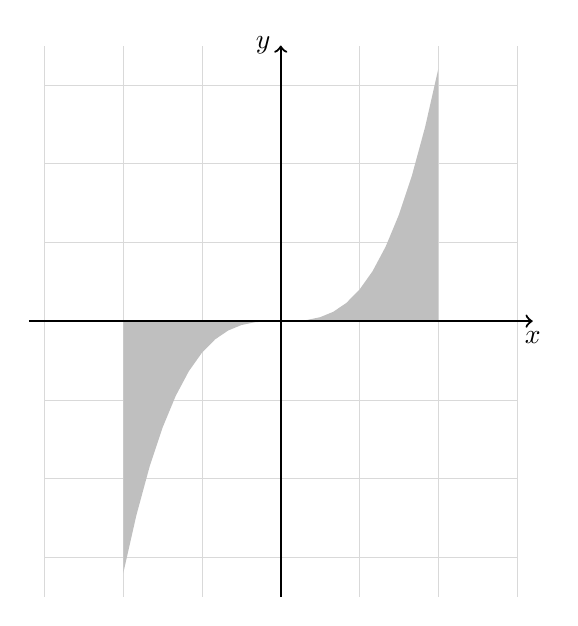
\begin{tikzpicture}

  \draw[very thin, gray!30, step = 1cm] (-3, -3.5) grid (3, 3.5);
  \fill[lightgray, domain = -2 : 2, variable = \x]
    (-2, -3.2)
    -- plot ({\x}, {0.4 * \x * \x * \x })
    -- (2, 0)
    -- (-2, 0)
    -- cycle;

  \draw[thick] [->] (-3.2, 0) -- (3.2, 0) node[right, below] {\(x\)};
  \draw[thick] [->] (0, -3.5) -- (0, 3.5) node[above, left] {\(y\)};

\end{tikzpicture}
\caption{\(f(-x) = -f(x)\)}\label{fig:int-symm-seg-odd}
\end{subfigure}
\qquad
\begin{subfigure}[b]{0.4\textwidth}
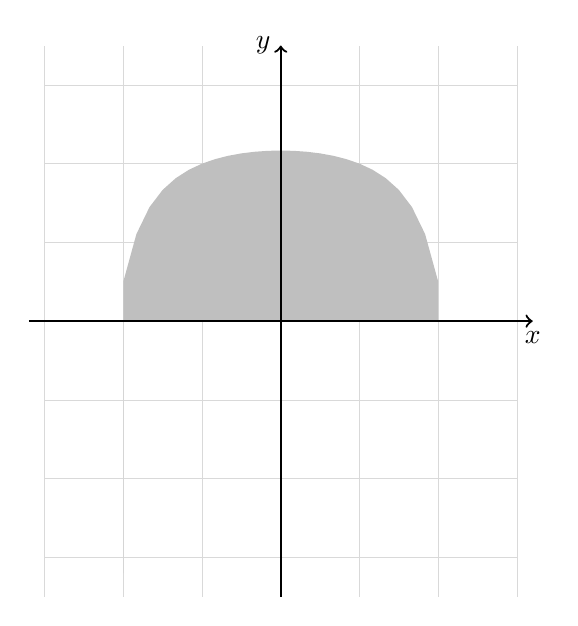
\begin{tikzpicture}

  \draw[very thin, gray!30, step = 1cm] (-3, -3.5) grid (3, 3.5);
  \fill[lightgray, domain = -2 : 2, variable = \x]
    (-2, -3.2)
    -- plot ({\x}, {(\x * \x - 1) / (\x * \x - 6) + 2})
    -- (2, 0)
    -- (-2, 0)
    -- cycle;

  \draw[thick] [->] (-3.2, 0) -- (3.2, 0) node[right, below] {\(x\)};
  \draw[thick] [->] (0, -3.5) -- (0, 3.5) node[above, left] {\(y\)};

\end{tikzpicture}
\caption{\(f(-x) = f(x)\)}\label{fig:int-symm-seg-even}
\end{subfigure}

\end{figure}
